\documentclass[conference]{IEEEtran}
\IEEEoverridecommandlockouts
% The preceding line is only needed to identify funding in the first footnote. If that is unneeded, please comment it out.
%Template version as of 6/27/2024

\usepackage{float}
\usepackage{cite}
\usepackage{amsmath,amssymb,amsfonts}
\usepackage{algorithmic}
\usepackage{graphicx}
\usepackage{textcomp}
\usepackage{xcolor}
\usepackage[dvipsnames]{xcolor}
\usepackage{hyperref}
\usepackage[utf8]{inputenc}
\usepackage[greek,english]{babel}
\usepackage{alphabeta}
\usepackage{listings}
\hypersetup{colorlinks=true, linkcolor=black, urlcolor=black, citecolor=black}

\lstset{
  language=VHDL,
  basicstyle=\ttfamily\small,
  keywordstyle=\color{blue},
  commentstyle=\color{gray},
  stringstyle=\color{red},
  numbersep=5pt,
  frame=single,
  captionpos=b,
  breaklines=true,
  tabsize=1
}

\def\BibTeX{{\rm B\kern-.05em{\sc i\kern-.025em b}\kern-.08em
    T\kern-.1667em\lower.7ex\hbox{E}\kern-.125emX}}
\begin{document}

\title{EchoLite: Υλοποίηση Συστήματος Μέτρησης Απόστασης με Υπερηχητικό Αισθητήρα σε FPGA Χρησιμοποιώντας VHDL}

\author{
	\IEEEauthorblockN{Ιορδάνης Κωστελίδης}
	\IEEEauthorblockA{
		\textit{Πρόγραμμα Μεταπτυχιακών Σπουδών στη Ρομποτική}\\
		\textit{Τμήμα Μηχανικών Πληροφορικής, Υπολογιστών και Τηλεπικοινωνιών}\\
		\textit{Πολυτεχνική Σχολή}\\
		\textit{Διεθνές Πανεπιστήμιο της Ελλάδος}\\
		Σέρρες, Ελλάδα \\
		iordkost@ihu.gr
	}
}

\maketitle

\begin{abstract}
	Το EchoLite είναι ένα σύστημα που μετρά αποστάσεις με τη βοήθεια υπερηχητικού αισθητήρα. Έχει φτιαχτεί πάνω σε πλακέτα FPGA (Intel DE10-Lite) και λειτουργεί εξ ολοκλήρου με κώδικα VHDL.
\end{abstract}

\begin{IEEEkeywords}
	FPGA, VHDL, distance measurement, ultrasonic sensor, HC-SR04, DE10-Lite, Altera MAX 10, embedded systems, digital design, real-time systems
\end{IEEEkeywords}

\section{Εισαγωγή}
Το EchoLite αποτελεί ένα σύστημα μέτρησης αποστάσεων εμποδείων σε  \texttt{FPGA}, το οποίο μπορεί να βρει εφαρμογή σε διάφορους τομείς όπως η ρομποτική, τα αυτόνομα οχήματα και τα ενσωματωμένα συστήματα ελέγχου. Η δυνατότητα γρήγορης μέτρησης απόστασης σε πραγματικό χρόνο είναι σημαντική για την αποφυγή εμποδίων, την πλοήγηση και την αυτοματοποίηση. Επιπλέον, η υλοποίηση σε  \texttt{FPGA} προσφέρει πλεονεκτήματα όπως ταχύτητα και δυνατότητα παραμετροποίησης, καθιστώντας το σύστημα χρήσιμο και σ' άλλες περιπτώσεις όπου απαιτείται επεξεργασία σήματος χωρίς μικροελεγκτή.

\begin{figure}[H]
	\centerline{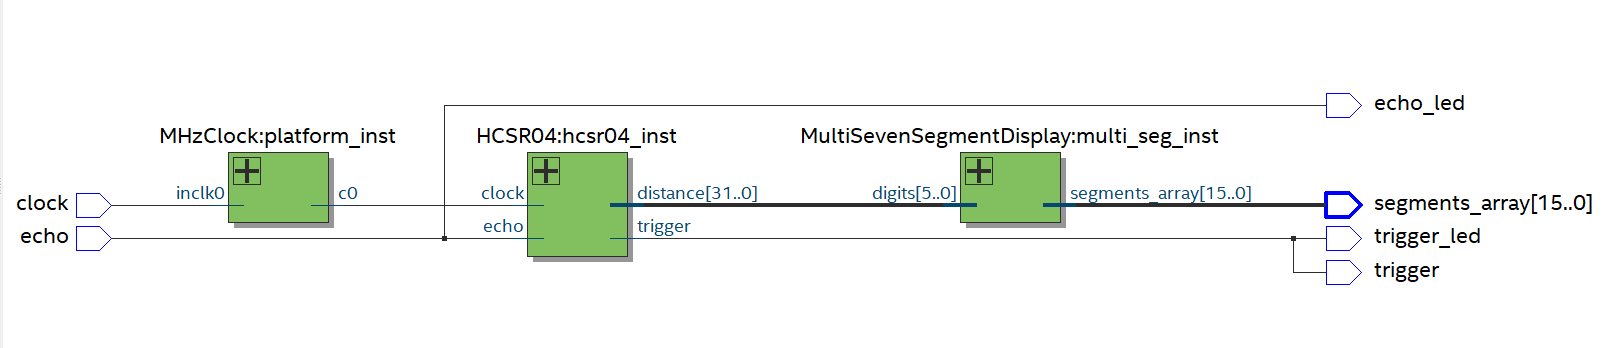
\includegraphics[width=0.4\textwidth]{assets/echolite.png}}
	\caption{Διάγραμμα του EchoLite.}
\end{figure}

\section{Προδιαγραφές}
Το τελικό σύστημα πρέπει να:
\begin{itemize}
    \item Μετρά την απόσταση χρησιμοποιώντας τον υπερηχητικό αισθητήρα  \texttt{HC-SR04}.
    \item Υλοποιηθεί πλήρως σε γλώσσα περιγραφής υλικού ( \texttt{VHDL}) πάνω στην πλακέτα  \texttt{DE10-Lite}
    \item Εμφανίζει την απόσταση μέσω των ενδεικτών 7 τμημάτων (\texttt{Seven Segment Displays}).
\end{itemize}

\section{Λίστα Υλικών}
\subsection{Lenovo Legion Y530-15ICH}
\begin{figure}[H]
	\centerline{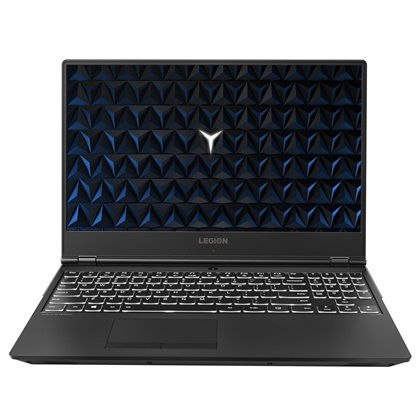
\includegraphics[width=0.4\textwidth]{assets/legion.jpg}}
	\caption{Υπολογιστής Lenovo Legion Y530-15INC.}
\end{figure}
Χρησιμοποιείται ως ο κύριος υπολογιστής για την ανάπτυξη του VHDL αλλα και την εκτέλεση δοκιμών (test bench) στο Quartus.

\subsection{DE10-Lite}
\begin{figure}[H]
	\centerline{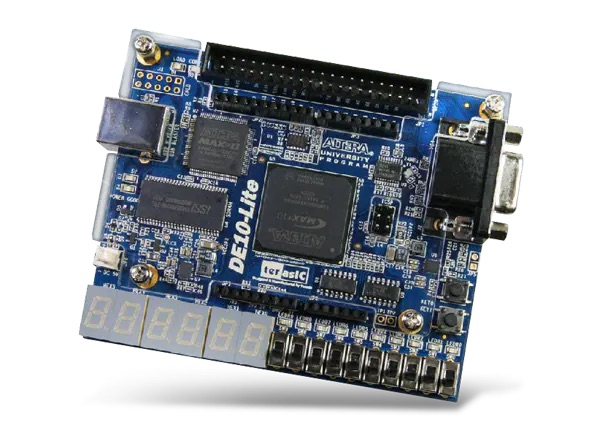
\includegraphics[width=0.4\textwidth]{assets/de10lite.jpeg}}
	\caption{Πλατφόρμα DE10-Lite.}
\end{figure}
Αναπτυξιακή πλατφόρμα FPGA της Intel (Altera).

\subsection{HC SR-04}
\begin{figure}[H]
	\centerline{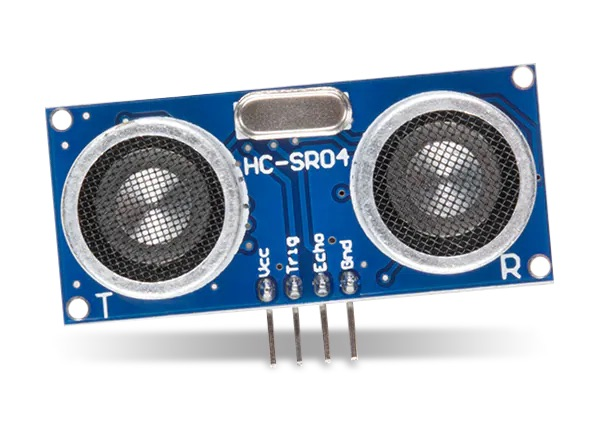
\includegraphics[width=0.4\textwidth]{assets/hcsr04.jpeg}}
	\caption{Αισθητήρας HC SR-04.}
\end{figure}
Αισθητήρας υπερήχων που χρησιμοποιείται για τη μέτρηση αποστάσεων.

\subsection{Καλώδια}
\begin{figure}[H]
	\centerline{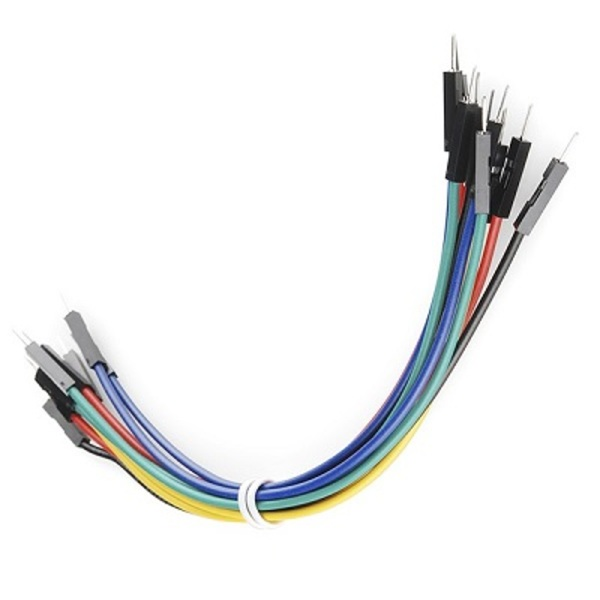
\includegraphics[width=0.4\textwidth]{assets/cables.jpg}}
	\caption{Καλώδια συνδεσης.}
\end{figure}
Χρησιμοποιούνται για τη σύνδεση των επιμέρους εξαρτημάτων μεταξύ τους, εξασφαλίζοντας τη σωστή μεταφορά σημάτων και τροφοδοσίας.

\subsection{Breadboard}
\begin{figure}[H]
	\centerline{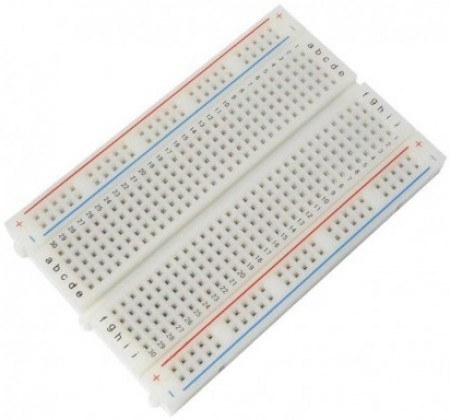
\includegraphics[width=0.4\textwidth]{assets/breadboard.jpg}}
	\caption{Πλακέτα δοκιμών πρωτότυπων κυκλωμάτων.}
\end{figure}
Πλακέτα για γρήγορη και εύκολη κατασκευή κυκλωμάτων χωρίς την ανάγκη συγκόλλησης. Χρησιμοποιείται για τη συναρμολόγηση του πρωτότυπου του συστήματος.

\section{Βασικές σχεδιαστικές επιλογές}
Για την υλοποίηση επιλέχθηκε η πλακέτα  \texttt{DE10-Lite}\cite{de10lite} με τον  \texttt{Altera MAX 10}\cite{de10litemanual}, ο υπερηχητικός αισθητήρας  \texttt{HC-SR04}\cite{hcsr04} και οι ενδείκτες 7 τμημάτων του  \texttt{DE10-Lite}\cite{de10litemanual}, καθώς ήταν μέρος της εκφώνησης της εργασίας.

\section{Περιγραφή υλοποίησης}
Η υλοποίηση έγινε με το λογισμικό Quartus\cite{quartus} και χωρίστηκε σε τέσσερα μικρότερα project:
\begin{itemize}
    \item \textbf{Seven Segment Display}: Διαχείριση και οδήγηση ενός ενδείκτη 7 τμημάτων για την απεικόνιση ενός ψηφίου.
    \item \textbf{Multi Seven Segment Display}: Επέκταση της προηγούμενης υλοποίησης για την ταυτόχρονη εμφάνιση πολλαπλών ψηφίων, απαραίτητη για την παρουσίαση μεγαλύτερων αριθμών.
    \item \textbf{HC-SR04}: Υλοποίηση του χρονισμού εκπομπής του \texttt{trigger} παλμού, υπολογισμό της διάρκειας του echo παλμού και μέτρησης απόστασης με βάση της διάρκεια του \texttt{echo} παλμού.
    \item \textbf{EchoLite}: Συνδυασμός των παραπάνω σε ένα ολοκληρωμένο σύστημα, με σωστή διαχείριση εισόδων/εξόδων και συγχρονισμό.
\end{itemize}

\section{Υλοποίηση}
\subsection{Seven Segment Display}
Ο παρακάτω \texttt{VHDL} κώδικας υλοποιεί μία μονάδα \texttt{SevenSegmentDisplay}, η οποία εμφανίζει έναν δυαδικό αριθμό \texttt{4-bit} σε ενδείκτη 7 τμημάτων.

\begin{itemize}
    \item \texttt{digit}: Είσοδος \texttt{4-bit}, που αντιπροσωπεύει το ψηφίο (0–9) σε δυαδική μορφή.
    \item \texttt{segments}: Έξοδος \texttt{8-bit} για τα 7 τμήματα της οθόνης και την τελεία.
\end{itemize}

\begin{lstlisting}[caption=Seven Segment Display VHDL Code, label=lst:ssd]
LIBRARY IEEE;
USE IEEE.STD_LOGIC_1164.ALL;

-- Interface
ENTITY SevenSegmentDisplay IS
	PORT (
		digit : IN STD_LOGIC_VECTOR (3 DOWNTO 0);
		segments : OUT STD_LOGIC_VECTOR (7 DOWNTO 0)
	);
END;

-- Implementation
ARCHITECTURE SevenSegmentDisplayArch OF SevenSegmentDisplay IS
BEGIN
	PROCESS(digit)
	BEGIN
		CASE digit IS
			WHEN "0000" => segments <= "11000000"; -- 0
			WHEN "0001" => segments <= "11111001"; -- 1
			WHEN "0010" => segments <= "10100100"; -- 2
			WHEN "0011" => segments <= "10110000"; -- 3
			WHEN "0100" => segments <= "10011001"; -- 4
			WHEN "0101" => segments <= "10010010"; -- 5
			WHEN "0110" => segments <= "10000010"; -- 6
			WHEN "0111" => segments <= "11111000"; -- 7
			WHEN "1000" => segments <= "10000000"; -- 8
			WHEN "1001" => segments <= "10010000"; -- 9
			WHEN OTHERS => segments <= "11111111"; -- blank
		END CASE;
	END PROCESS;
END;
\end{lstlisting}

\subsection{Multi Seven Segment Display}
Ο παρακάτω \texttt{VHDL} κώδικας υλοποιεί μία μονάδα \texttt{MultiSevenSegmentDisplay}, η οποία μετατρέπει έναν ακέραιο δυαδικό αριθμό σε ακολουθία δεκαδικών ψηφίων και προβάλλει καθένα από αυτά σε ενδείκτες 7 τμημάτων μέσω της μονάδας \texttt{SevenSegmentDisplay}.

\begin{itemize}
    \item \texttt{digits}: Είσοδος, που αντιπροσωπεύει τον αριθμό προς εμφάνιση σε δυαδική μορφή. Το μεγεθός της σε \texttt{bits} καθορίζεται σταθερά.
    \item \texttt{segments\_array}: Έξοδος, που περιέχει τα \texttt{bits} όλων των 7-τμηματικών οθονών.
\end{itemize}

\begin{lstlisting}[caption=Multi Seven Segment Display VHDL Code, label=lst:mssd]
LIBRARY IEEE;
USE IEEE.STD_LOGIC_1164.ALL;
USE IEEE.NUMERIC_STD.ALL;

-- Interface
ENTITY MultiSevenSegmentDisplay IS
    GENERIC (
        INPUT_WIDTH : INTEGER := 6;
        NUM_DIGITS : INTEGER := 2
    );
    PORT (
        digits : IN STD_LOGIC_VECTOR(INPUT_WIDTH - 1 DOWNTO 0);
        segments_array : OUT STD_LOGIC_VECTOR(NUM_DIGITS * 8 - 1 DOWNTO 0)
    );
END ENTITY;

-- Implementation
ARCHITECTURE MultiSevenSegmentDisplayArch OF MultiSevenSegmentDisplay IS

    COMPONENT SevenSegmentDisplay
        PORT (
            digit : IN STD_LOGIC_VECTOR (3 DOWNTO 0);
            segments : OUT STD_LOGIC_VECTOR (7 DOWNTO 0)
        );
    END COMPONENT;
	 
	 TYPE LOGIC_VECTOR_ARRAY IS ARRAY (0 TO NUM_DIGITS - 1) OF STD_LOGIC_VECTOR(3 DOWNTO 0);
	 
    SIGNAL binary_value_sig : UNSIGNED(INPUT_WIDTH - 1 DOWNTO 0);
    SIGNAL binary_digits_sig : LOGIC_VECTOR_ARRAY;
    SIGNAL segments_sig : STD_LOGIC_VECTOR(NUM_DIGITS * 8 - 1 DOWNTO 0);

BEGIN

    binary_value_sig <= UNSIGNED(digits);

    -- Split digits
    PROCESS(binary_value_sig)
        VARIABLE value : INTEGER;
    BEGIN
        value := TO_INTEGER(binary_value_sig);
        FOR i IN 0 TO NUM_DIGITS - 1 LOOP
            binary_digits_sig(i) <= STD_LOGIC_VECTOR(TO_UNSIGNED(value MOD 10, 4));
            value := value / 10;
        END LOOP;
    END PROCESS;

    -- Generate segment displays
    gen_segments : FOR i IN 0 TO NUM_DIGITS - 1
		 GENERATE SIGNAL seg : STD_LOGIC_VECTOR(7 DOWNTO 0);
		 BEGIN
			  seg_inst : SevenSegmentDisplay
					PORT MAP (
						 digit => binary_digits_sig(i),
						 segments => seg
					);
			  segments_sig((i + 1) * 8 - 1 DOWNTO i * 8) <= seg;
		 END GENERATE;

    segments_array <= segments_sig;

END ARCHITECTURE;
\end{lstlisting}

\subsection{HCSR04}
Ο παρακάτω \texttt{VHDL} κώδικας υλοποιεί μία μονάδα \texttt{HCSR04}, η οποία διαχειρίζεται τον υπερηχητικό αισθητήρα απόστασης \texttt{HC-SR04}. Η μονάδα ενεργοποιεί τον αισθητήρα με παλμό \texttt{trigger} και μετρά τη διάρκεια του σήματος \texttt{echo}, \\υπολογίζοντας την απόσταση βάσει του χρόνου επιστροφής του υπερηχητικού κύματος.

\begin{itemize}
    \item \texttt{clock}: Σήμα ρολογιού για συγχρονισμό της μέτρησης.
    \item \texttt{echo}: Είσοδος από τον αισθητήρα \texttt{HC-SR04}
    \item \texttt{trigger}: Έξοδος που στέλνει παλμό ενεργοποίησης προς τον αισθητήρα.
    \item \texttt{distance}: Έξοδος που είναι η απόσταση σε εκατοστά.
\end{itemize}

Η μονάδα στέλνει παλμό \texttt{trigger} διάρκειας 10 κύκλων ρολογιού. Σύμφωνα με τις οδηγίες του HC-SR04\cite{hcsr04}, ο παλμός αυτός πρέπει να διαρκεί \textbf{10 microseconds}, επομένως η συχνότητα του ρολογιού πρέπει να είναι \textbf{1 MHz}, έτσι ώστε ο κάθε κύκλος ρολογιού να είναι \texttt{1 microsecond}.

Στη συνέχεια, η μονάδα μετρά τους κύκλους ρολογιού όσο το \texttt{echo} είναι ενεργό. Όταν το \texttt{echo} μηδενιστεί, αποθηκεύεται η διάρκεια και υπολογίζεται η απόσταση. \\

Η αρχική εξίσωση για την απόσταση που διανύει είναι:

\[
\text{απόσταση} = \frac{t_{\text{echo}} \cdot v_{\text{ήχου}}}{2}
\]

όπου:
\begin{itemize}
    \item \( t_{\text{echo}} \): ο συνολικός χρόνος μετάδοσης και επιστροφής του ηχητικού κύματος (σε μικροδευτερόλεπτα),
    \item \( v_{\text{ήχου}} \): η ταχύτητα του ήχου στον αέρα, περίπου \(343\ \text{m/s} = 0.0343\ \text{cm}/\mu s\).
\end{itemize}

Επειδή ο ήχος διανύει τη διπλάσια απόσταση (προς τον στόχο και πίσω), διαιρούμε με το 2:

\[
\text{απόσταση (σε cm)} = \frac{t_{\text{echo}} \cdot 0.0343}{2}
= t_{\text{echo}} \cdot 0.01715
\]

Προσεγγίζοντας:

\[
\text{απόσταση} \approx t_{\text{echo}} \cdot \frac{17}{1000}
\]

Άρα, ο απλοποιημένος τύπος είναι:

\[
\text{απόσταση} \approx \frac{t_{\text{echo}} \cdot 17}{1000}
\]

\begin{lstlisting}[caption=HC SR-04 VHDL Code, label=lst:hcsr04]
LIBRARY IEEE;
USE IEEE.STD_LOGIC_1164.ALL;
USE IEEE.STD_LOGIC_UNSIGNED.ALL;

-- Interface
ENTITY HCSR04 IS
	PORT (
		clock    : IN STD_LOGIC;
		echo		: IN STD_LOGIC;
		trigger  : OUT STD_LOGIC;
		distance : OUT INTEGER
	);
END ENTITY;

-- Implementation
ARCHITECTURE HCSR04Arch OF HCSR04 IS
	SIGNAL trigger_sig : STD_LOGIC := '0';
	SIGNAL distance_sig : INTEGER := 0;
	SIGNAL echo_time : INTEGER := 0;
BEGIN
	PROCESS(clock)
		VARIABLE trigger_count, echo_count : INTEGER := 0;
		VARIABLE can_calculate : STD_LOGIC := '1';
	BEGIN
		IF RISING_EDGE(clock) THEN
			IF trigger_count = 0 THEN
				trigger_sig <= '1';
			ELSIF trigger_count = 10 THEN
				trigger_sig <= '0';
				can_calculate := '1';
			ELSIF trigger_count = 200000 THEN
				trigger_count := 0;
				trigger_sig <= '1';
			END IF;
			trigger_count := trigger_count + 1;

			IF echo = '1' THEN
				IF echo_count < 3706 THEN
					echo_count := echo_count + 1;
				END IF;
			ELSIF echo = '0' AND can_calculate = '1' THEN
				echo_time <= echo_count;
				echo_count := 0;
				can_calculate := '0';
			END IF;

			distance_sig <= (echo_time * 17) / 1000;
		END IF; 
	END PROCESS;

	trigger <= trigger_sig;
	distance <= distance_sig;
END ARCHITECTURE;
\end{lstlisting}

\subsection{EchoLite}
Ο παρακάτω \texttt{VHDL} κώδικας υλοποιεί την κεντρική μονάδα \texttt{EchoLite}, η οποία χρησιμοποιεί τον αισθητήρα απόστασης \texttt{HC-SR04} και απεικονίζει την απόσταση δύο ενδείκτες 7 τμημάτων.

\begin{itemize}
    \item \texttt{clock}: Κύριο σήμα ρολογιού συστήματος (\texttt{50MHz}), χρησιμοποιείται ως είσοδος στη μονάδα παραγωγής ρολογιού \texttt{1MHz}.
    \item \texttt{echo}, \texttt{trigger}: Σήματα που συνδέονται με τον αισθητήρα \texttt{HC-SR04}.
    \item \texttt{segments\_array}: Έξοδος προς τους 2 εκδείκτες 7 τμημάτων.
    \item \texttt{echo\_led}, \texttt{trigger\_led}: Έξοδοι LED για τα σήματα \texttt{echo} και \texttt{trigger}, για λόγους \texttt{debug}.
\end{itemize}

Η αρχιτεκτονική περιλαμβάνει τις εξής υπομονάδες:

\begin{itemize}
    \item \textbf{\texttt{MHzClock}}: Παράγει ρολόι \texttt{1MHz} από το εισερχόμενο ρολόι των \texttt{50MHz}, απαραίτητο για την λειτουργία του \texttt{HC-SR04}. Το ρολόι αυτό έγινε μέσα από το \texttt{IP Catalogue} ως προραρμοσμένο \texttt{ALTPLL}\cite{altpll} με είσοδο \texttt{50MHz} και έξοδο \texttt{1MHz}.
    
    \item \textbf{\texttt{HCSR04}}: Διαχειρίζεται τον αισθητήρα απόστασης. Παράγει το σήμα \texttt{trigger}, μετρά τη διάρκεια του \texttt{echo} και υπολογίζει την απόσταση σε εκατοστά.

    \item \textbf{\texttt{MultiSevenSegmentDisplay}}: Εμφανίζει την απόσταση σε 2 ενδείκτες 7 τμημάτων.
\end{itemize}

Το σήμα \texttt{distance\_sig}, που παρέχεται από τον αισθητήρα, μετατρέπεται σε \texttt{STD\_LOGIC\_VECTOR} και οδηγείται στην οθόνη μέσω της μονάδας \texttt{MultiSevenSegmentDisplay}. Παράλληλα, τα σήματα \texttt{echo} και \texttt{trigger} προβάλλονται και μέσω \texttt{LED} για οπτική επιβεβαίωση της λειτουργίας του αισθητήρα (\texttt{debug}).

\begin{lstlisting}[caption=EchoLight VHDL Code, label=lst:el]
LIBRARY IEEE;
USE IEEE.STD_LOGIC_1164.ALL;
USE IEEE.NUMERIC_STD.ALL;

-- Interface
ENTITY EchoLite IS
	PORT (
		clock    : IN STD_LOGIC;
		echo		: IN STD_LOGIC;
		trigger  : OUT STD_LOGIC;
		segments_array : OUT STD_LOGIC_VECTOR(2 * 8 - 1 DOWNTO 0);
		
		echo_led : OUT STD_LOGIC;
		trigger_led : OUT STD_LOGIC
	);
END ENTITY;

-- Implementation
ARCHITECTURE EchoLiteArch OF EchoLite IS

-- Custom Clock
COMPONENT MHzClock
	PORT
	(
		inclk0		: IN STD_LOGIC  := '0';
		c0				: OUT STD_LOGIC 
	);
END COMPONENT;

-- Multiple Seven-Sgement Display Support
COMPONENT MultiSevenSegmentDisplay
	PORT (
	  digits : IN STD_LOGIC_VECTOR(6 - 1 DOWNTO 0);
	  segments_array : OUT STD_LOGIC_VECTOR(2 * 8 - 1 DOWNTO 0)
	);
END COMPONENT;

-- HC SR-04 Support
COMPONENT HCSR04
	PORT (
		clock    : IN STD_LOGIC;
		echo		: IN STD_LOGIC;
		trigger  : OUT STD_LOGIC;
		distance : OUT INTEGER
	);
END COMPONENT;

SIGNAL clock_sig : STD_LOGIC;
SIGNAL digits_sig : STD_LOGIC_VECTOR(6 - 1 DOWNTO 0);
SIGNAL distance_sig : INTEGER;
SIGNAL trigger_sig : STD_LOGIC;

BEGIN

platform_inst :  MHzClock
	PORT MAP (
		inclk0		=> clock,
		c0				=> clock_sig
	);

multi_seg_inst : MultiSevenSegmentDisplay
	PORT MAP (
		digits			=> digits_sig,
		segments_array	=> segments_array
	);
	
hcsr04_inst : HCSR04
	PORT MAP (
		clock		=> clock_sig,
		echo		=> echo,
		trigger	=> trigger_sig,
		distance	=> distance_sig
	);

digits_sig <= STD_LOGIC_VECTOR(TO_UNSIGNED(distance_sig, 6));
echo_led <= echo;
trigger <= trigger_sig;
trigger_led <= trigger_sig;
	
END ARCHITECTURE;
\end{lstlisting}

\section{Πόροι υλοποίησης}
Στην αναφορά σύνθεσης από το \textit{Quartus} περιλαμβάνονται:
\begin{itemize}
    \item Αριθμός χρησιμοποιημένων \textbf{Logic Elements (LEs)} : 984
    \item Αριθμός \textbf{καταχωρητών (Registers)} : 104
    \item Αριθμός \textbf{pins} που χρησιμοποιήθηκαν) : 21
    \item Αριθμός \textbf{PPLs} : 1
\end{itemize}

\section{Δοκιμές}
\subsection{SevenSegmentDisplay}

Προσομοίωση
\begin{figure}[H]
	\centerline{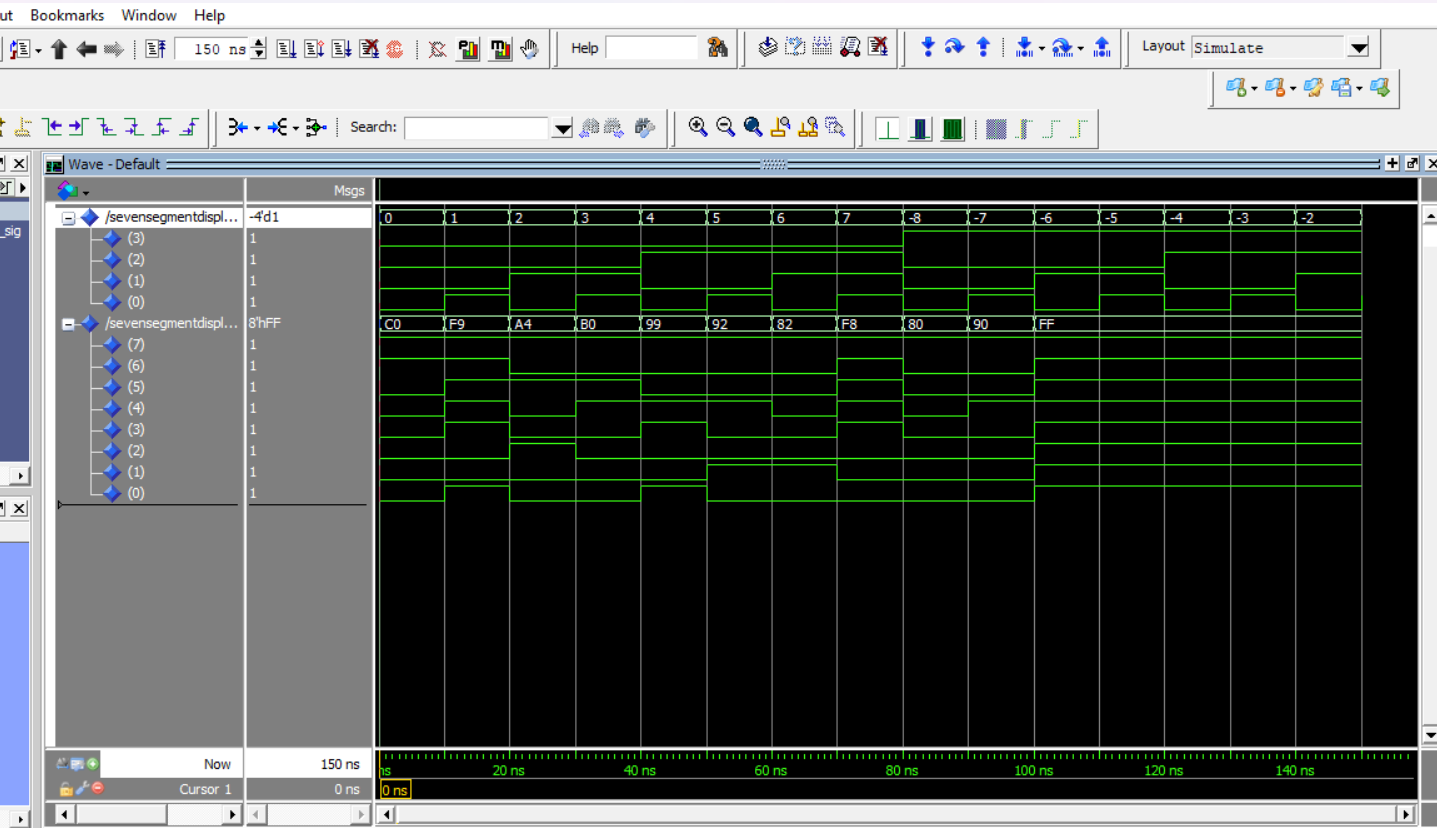
\includegraphics[width=0.4\textwidth]{assets/ssd-tb.png}}
	\caption{Προσομοίωση του SevenSegmentDisplay}
\end{figure}

Πραγματικό
\begin{figure}[H]
	\centerline{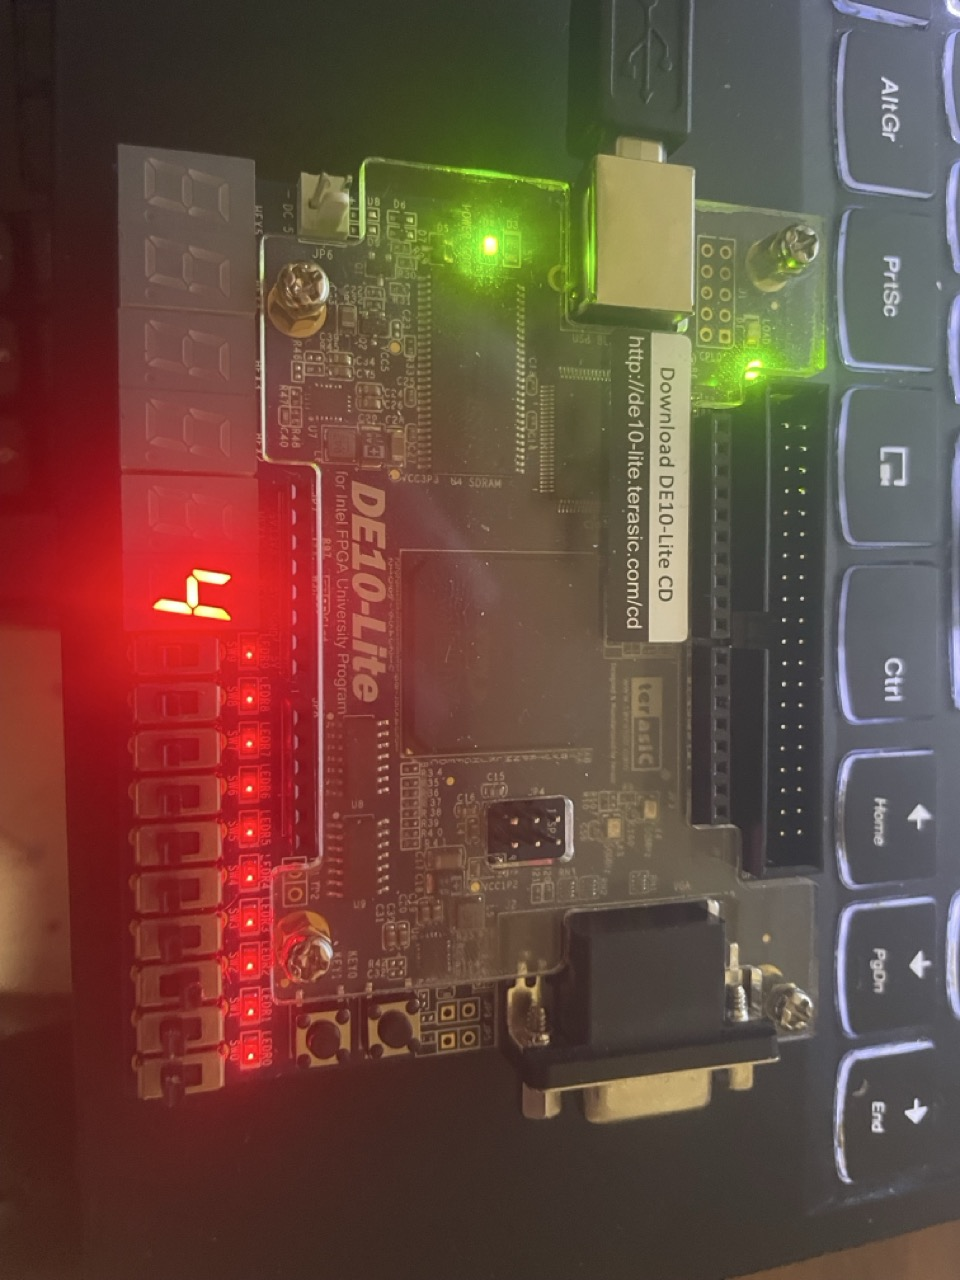
\includegraphics[angle=90, width=0.4\textwidth]{assets/ssd-real.jpeg}}
	\caption{Πραγματική χρήση του SevenSegmentDisplay.}
\end{figure}

\subsection{MultiSevenSegmentDisplay}

Προσομοίωση
\begin{figure}[H]
	\centerline{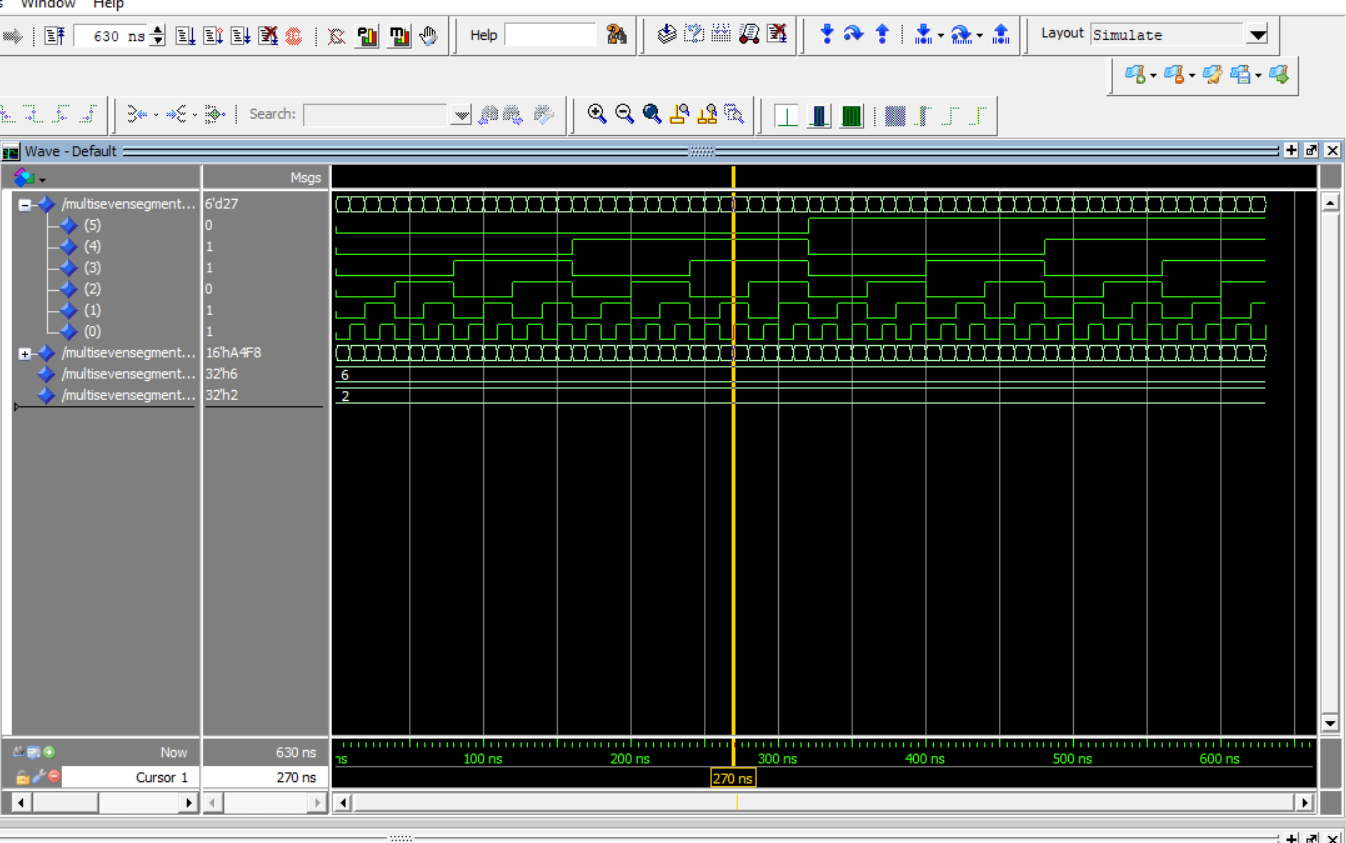
\includegraphics[width=0.4\textwidth]{assets/mssd-tb.png}}
	\caption{Προσομοίωση του MultiSevenSegmentDisplay}
\end{figure}

Πραγματικό
\begin{figure}[H]
	\centerline{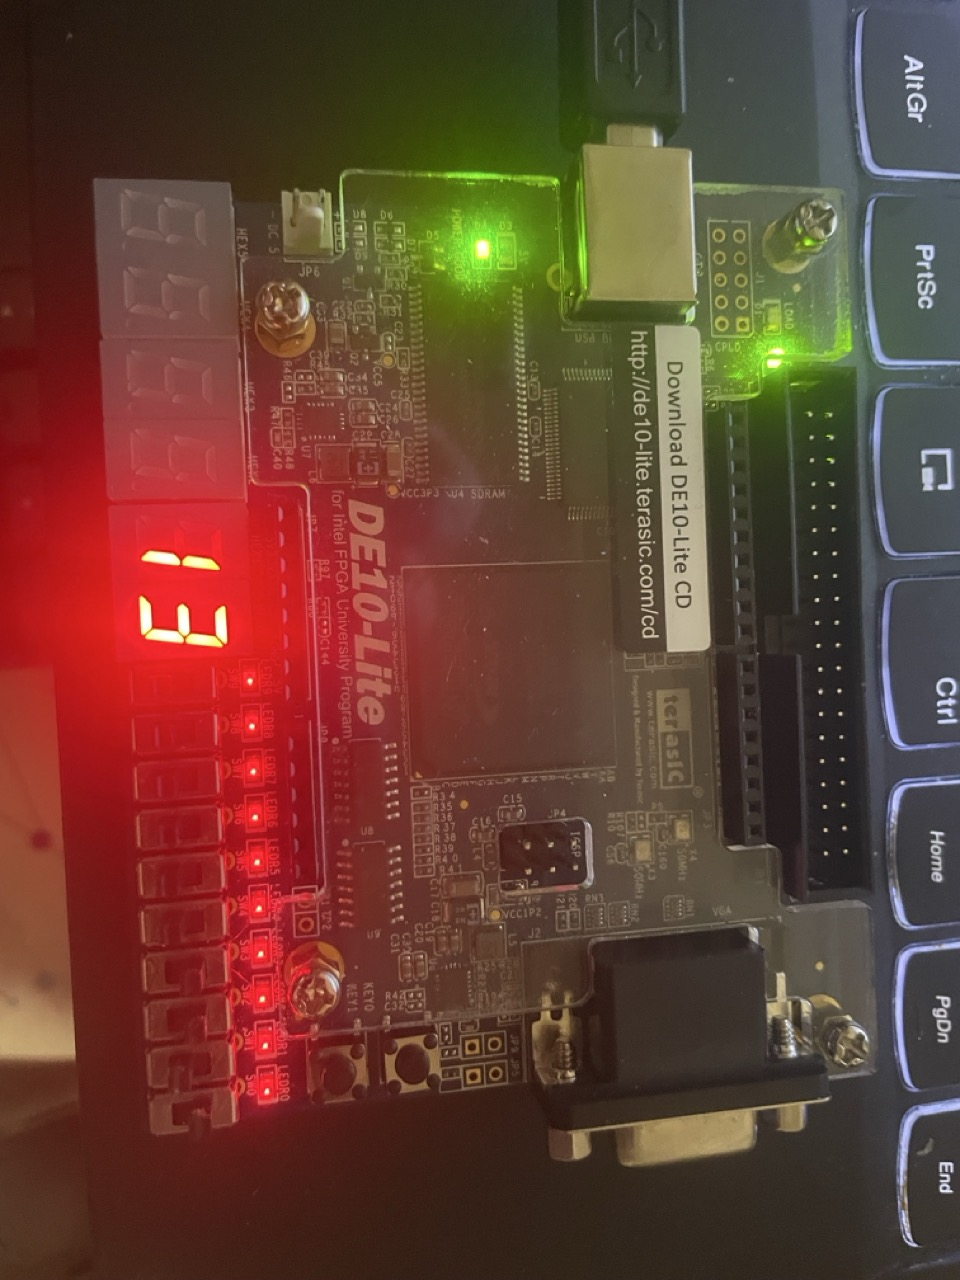
\includegraphics[angle=90, width=0.4\textwidth]{assets/mssd-real.jpeg}}
	\caption{Πραγματική χρήση του MultiSevenSegmentDisplay.}
\end{figure}

\subsection{HC SR-04}

Προσομοίωση
\begin{figure}[H]
	\centerline{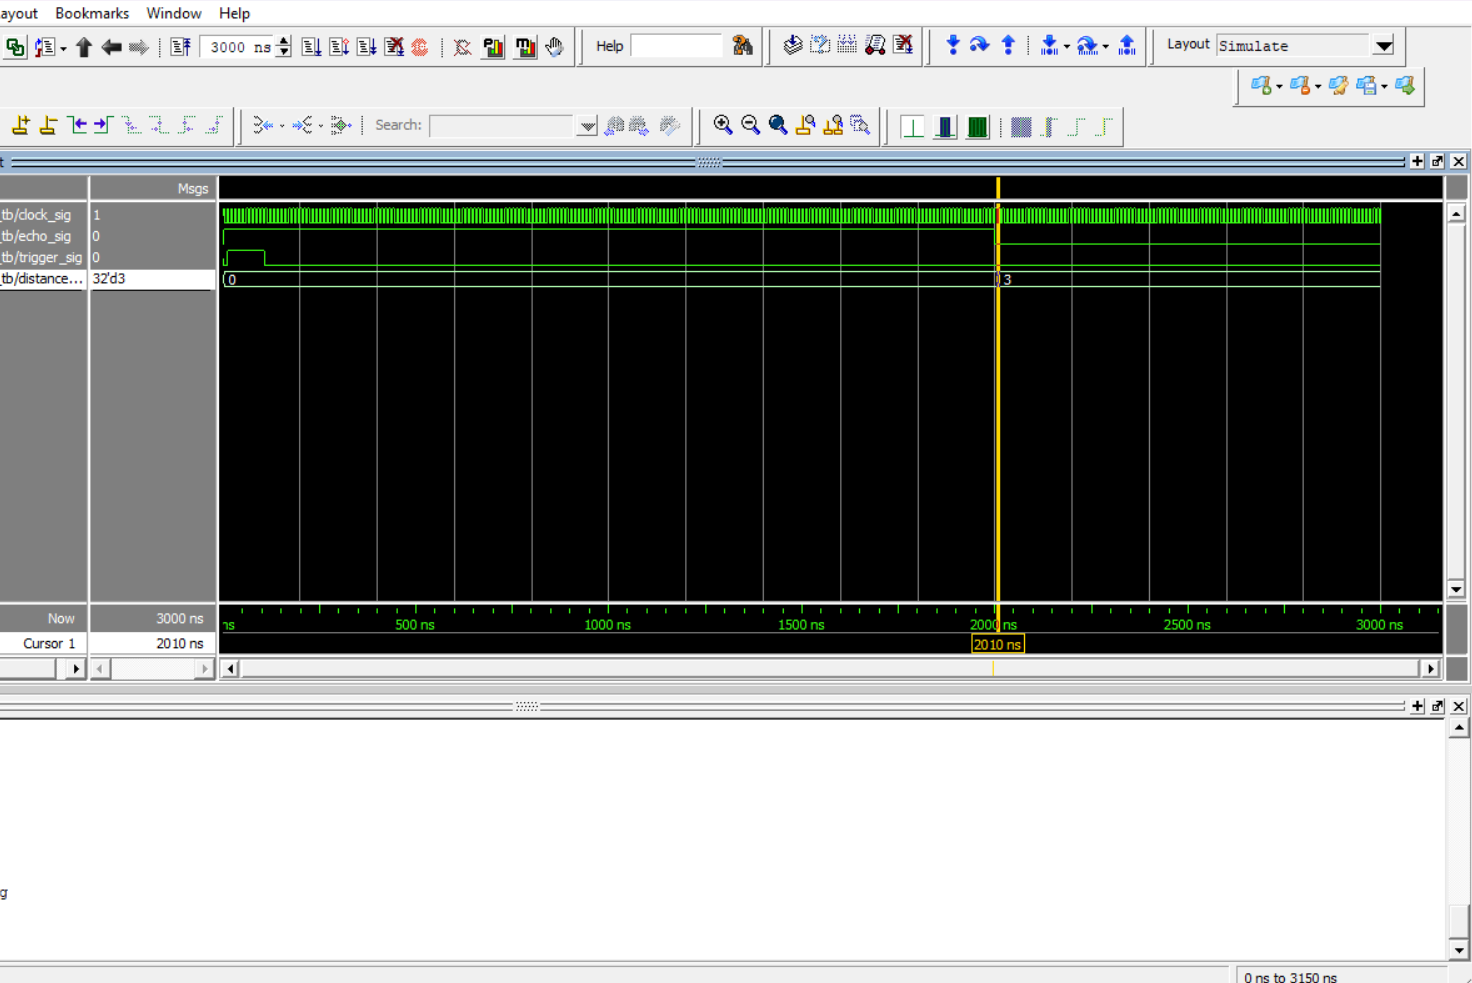
\includegraphics[width=0.4\textwidth]{assets/hcsr04-tb.png}}
	\caption{Προσομοίωση του HC SR-03}
\end{figure}

\subsection{EchoLite}

Πραγματικό
\begin{figure}[H]
	\centerline{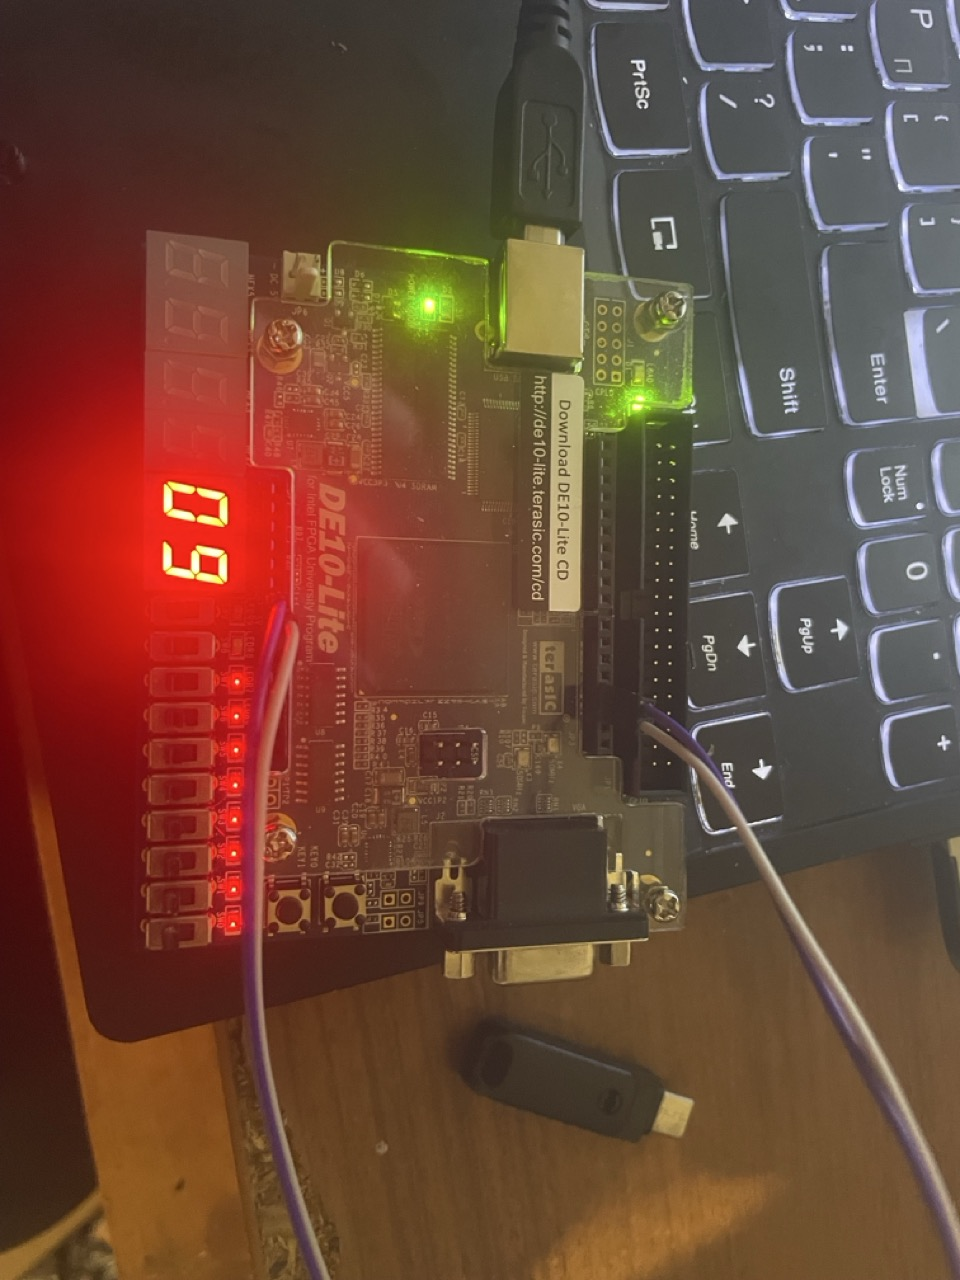
\includegraphics[angle=90, width=0.4\textwidth]{assets/echolite-real.jpeg}}
	\caption{Πραγματική χρήση του EchoLite.}
\end{figure}

\section{Συμπεράσματα και μελλοντικές προοπτικές}
Το σύστημα \texttt{EchoLite} πέτυχε την μέτρηση αποστάσεων σε πραγματικό χρόνο, αποδεικνύοντας την αποτελεσματικότητα της χρήσης \texttt{FPGA} σε εφαρμογές αισθητήρων. Η διαίρεση σε ξεχωριστά \texttt{projects} διευκόλυνε την ανάπτυξη και τον έλεγχο του κάθε υποσυστήματος (test bench).
Τα πιο δύσκολα σημεία αφορούσαν τον ακριβή χρονικό συγχρονισμό των σημάτων και τη σωστή μέτρηση των παλμών για τον υπολογισμό της απόστασης. Η υλοποίηση βοήθησε στην κατανόηση ψηφιακών συστημάτων, VHDL και χρονισμού ρολογιών (\texttt{clocks}).
Μελλοντικά, το σύστημα μπορεί να επεκταθεί με επιπλέον αισθητήρες αλλά και την βελτιστοποίηση της ακρίβειας.

\section{Σχετικά με το έργο}
Αυτό το έργο πραγματοποιήθηκε στο πλαίσιο του μαθήματος Ρ203: Σχεδίαση Συστημάτων Υψηλών Επιδόσεων, στο μεταπτυχιακό πρόγραμμα στη Ρομποτική, που προσφέρεται από το Τμήμα Μηχανικών Πληροφορικής, Υπολογιστών και Τηλεπικοινωνιών του Διεθνούς Πανεπιστημίου της Ελλάδος.

 \enlargethispage{0mm}
\begin{thebibliography}{00}

\bibitem{de10lite}
``Terasic - DE Boards - MAX - DE10-Lite Development and Education Board,'' terasic.com.tw, 2025.\\
\url{https://www.terasic.com.tw/cgi-bin/page/archive.pl?Language=English&CategoryNo=234&No=1021} (accessed Jun. 25, 2025).

\bibitem{de10litemanual}
``DE10-Lite User Manual,'' terasic.com.tw, 2025.\\
\url{https://www.terasic.com.tw/cgi-bin/page/archive_download.pl?Language=English&No=1021&FID=a13a2782811152b477e60203d34b1baa} (accessed Jun. 25, 2025).

\bibitem{quartus}
``FPGA Design Software - Quartus\textsuperscript{\textregistered} Prime,'' intel.com, 2025.\\
\url{https://www.intel.com/content/www/us/en/products/details/fpga/development-tools/quartus-prime.html} (accessed Jun. 25, 2025).

\bibitem{hcsr04}
``Ultrasonic Ranging Module HC-SR04,'' sparkfun.com, 2025.\\
\url{https://cdn.sparkfun.com/datasheets/Sensors/Proximity/HCSR04.pdf} (accessed Jun. 25, 2025).

\bibitem{altpll}
``ALTPLL (Phase-Locked Loop) IP Core User Guide,'' intel.com, 2025.\\
\url{https://www.intel.com/content/www/us/en/docs/programmable/683732/17-0/altpll-phase-locked-loop-ip-core-user-guide.html} (accessed Jun. 25, 2025).

\end{thebibliography}

\end{document}